


\tikzset{every picture/.style={line width=0.75pt}} %set default line width to 0.75pt        

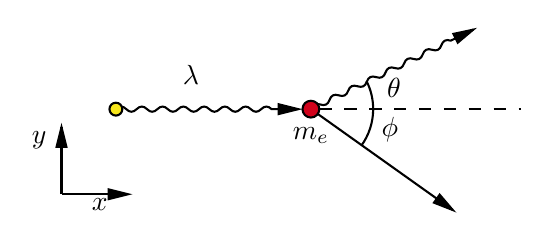
\begin{tikzpicture}[x=0.75pt,y=0.75pt,yscale=-1,xscale=1]
%uncomment if require: \path (0,300); %set diagram left start at 0, and has height of 300

%Straight Lines [id:da83534704962164] 
\draw    (86.2,110) .. controls (87.87,108.33) and (89.53,108.33) .. (91.2,110) .. controls (92.87,111.67) and (94.53,111.67) .. (96.2,110) .. controls (97.87,108.33) and (99.53,108.33) .. (101.2,110) .. controls (102.87,111.67) and (104.53,111.67) .. (106.2,110) .. controls (107.87,108.33) and (109.53,108.33) .. (111.2,110) .. controls (112.87,111.67) and (114.53,111.67) .. (116.2,110) .. controls (117.87,108.33) and (119.53,108.33) .. (121.2,110) .. controls (122.87,111.67) and (124.53,111.67) .. (126.2,110) .. controls (127.87,108.33) and (129.53,108.33) .. (131.2,110) .. controls (132.87,111.67) and (134.53,111.67) .. (136.2,110) .. controls (137.87,108.33) and (139.53,108.33) .. (141.2,110) .. controls (142.87,111.67) and (144.53,111.67) .. (146.2,110) .. controls (147.87,108.33) and (149.53,108.33) .. (151.2,110) .. controls (152.87,111.67) and (154.53,111.67) .. (156.2,110) .. controls (157.87,108.33) and (159.53,108.33) .. (161.2,110) -- (166.1,110) -- (174.1,110) ;
\draw [shift={(176.1,110)}, rotate = 180] [fill={rgb, 255:red, 0; green, 0; blue, 0 }  ][line width=0.08]  [draw opacity=0] (12,-3) -- (0,0) -- (12,3) -- cycle    ;
%Shape: Circle [id:dp7317051500535381] 
\draw  [fill={rgb, 255:red, 248; green, 231; blue, 28 }  ,fill opacity=1 ] (83.1,110) .. controls (83.1,108.29) and (84.49,106.9) .. (86.2,106.9) .. controls (87.91,106.9) and (89.3,108.29) .. (89.3,110) .. controls (89.3,111.71) and (87.91,113.1) .. (86.2,113.1) .. controls (84.49,113.1) and (83.1,111.71) .. (83.1,110) -- cycle ;
%Straight Lines [id:da8041402870048531] 
\draw    (180.15,109.95) .. controls (180.92,107.72) and (182.41,106.99) .. (184.64,107.75) .. controls (186.87,108.52) and (188.36,107.79) .. (189.13,105.56) .. controls (189.9,103.33) and (191.39,102.6) .. (193.62,103.36) .. controls (195.85,104.13) and (197.35,103.39) .. (198.12,101.16) .. controls (198.89,98.93) and (200.38,98.2) .. (202.61,98.97) .. controls (204.84,99.73) and (206.33,99) .. (207.1,96.77) .. controls (207.87,94.54) and (209.36,93.81) .. (211.59,94.57) .. controls (213.82,95.34) and (215.31,94.61) .. (216.08,92.38) .. controls (216.85,90.15) and (218.34,89.42) .. (220.57,90.18) .. controls (222.8,90.95) and (224.3,90.21) .. (225.07,87.98) .. controls (225.84,85.75) and (227.33,85.02) .. (229.56,85.79) .. controls (231.79,86.55) and (233.28,85.82) .. (234.05,83.59) .. controls (234.82,81.36) and (236.31,80.63) .. (238.54,81.39) .. controls (240.77,82.16) and (242.26,81.43) .. (243.03,79.2) .. controls (243.8,76.97) and (245.29,76.24) .. (247.52,77) -- (251.22,75.19) -- (258.4,71.68) ;
\draw [shift={(260.2,70.8)}, rotate = 153.94] [fill={rgb, 255:red, 0; green, 0; blue, 0 }  ][line width=0.08]  [draw opacity=0] (12,-3) -- (0,0) -- (12,3) -- cycle    ;
%Straight Lines [id:da15042270376010536] 
\draw  [dash pattern={on 4.5pt off 4.5pt}]  (184.2,109.95) -- (281.2,109.95) ;
%Straight Lines [id:da758135639798698] 
\draw    (180.15,109.95) -- (248.57,158.64) ;
\draw [shift={(250.2,159.8)}, rotate = 215.44] [fill={rgb, 255:red, 0; green, 0; blue, 0 }  ][line width=0.08]  [draw opacity=0] (12,-3) -- (0,0) -- (12,3) -- cycle    ;
%Shape: Arc [id:dp8030932944229654] 
\draw  [draw opacity=0] (206.95,96.45) .. controls (209,100.51) and (210.15,105.09) .. (210.15,109.95) .. controls (210.15,110.25) and (210.15,110.56) .. (210.14,110.86) -- (180.15,109.95) -- cycle ; \draw   (206.95,96.45) .. controls (209,100.51) and (210.15,105.09) .. (210.15,109.95) .. controls (210.15,110.25) and (210.15,110.56) .. (210.14,110.86) ;  
%Shape: Circle [id:dp06692297807124792] 
\draw  [fill={rgb, 255:red, 208; green, 2; blue, 27 }  ,fill opacity=1 ] (176.1,110) .. controls (176.1,107.76) and (177.91,105.95) .. (180.15,105.95) .. controls (182.39,105.95) and (184.2,107.76) .. (184.2,110) .. controls (184.2,112.24) and (182.39,114.05) .. (180.15,114.05) .. controls (177.91,114.05) and (176.1,112.24) .. (176.1,110) -- cycle ;
%Shape: Arc [id:dp7828883325590348] 
\draw  [draw opacity=0] (210.15,109.8) .. controls (210.15,109.87) and (210.15,109.93) .. (210.15,110) .. controls (210.15,116.56) and (208.05,122.62) .. (204.48,127.56) -- (180.15,110) -- cycle ; \draw   (210.15,109.8) .. controls (210.15,109.87) and (210.15,109.93) .. (210.15,110) .. controls (210.15,116.56) and (208.05,122.62) .. (204.48,127.56) ;  
%Straight Lines [id:da17293414654806027] 
\draw    (60,151) -- (92.2,151) ;
\draw [shift={(94.2,151)}, rotate = 180] [fill={rgb, 255:red, 0; green, 0; blue, 0 }  ][line width=0.08]  [draw opacity=0] (12,-3) -- (0,0) -- (12,3) -- cycle    ;
%Straight Lines [id:da3925593502685727] 
\draw    (60,151) -- (60,118.6) ;
\draw [shift={(60,116.6)}, rotate = 90] [fill={rgb, 255:red, 0; green, 0; blue, 0 }  ][line width=0.08]  [draw opacity=0] (12,-3) -- (0,0) -- (12,3) -- cycle    ;

% Text Node
\draw (117,87.4) node [anchor=north west][inner sep=0.75pt]    {$\lambda $};
% Text Node
\draw (180.15,117.45) node [anchor=north] [inner sep=0.75pt]    {$m_{e}$};
% Text Node
\draw (218.15,112.45) node [anchor=north] [inner sep=0.75pt]    {$\phi $};
% Text Node
\draw (220.17,93.78) node [anchor=north] [inner sep=0.75pt]    {$\theta $};
% Text Node
\draw (73.1,151.4) node [anchor=north west][inner sep=0.75pt]    {$x$};
% Text Node
\draw (44.2,119.4) node [anchor=north west][inner sep=0.75pt]    {$y$};


\end{tikzpicture}
